\subsection{Odometry Benchmark}\label{sec:odometry_images}
\begin{figure}[H]
    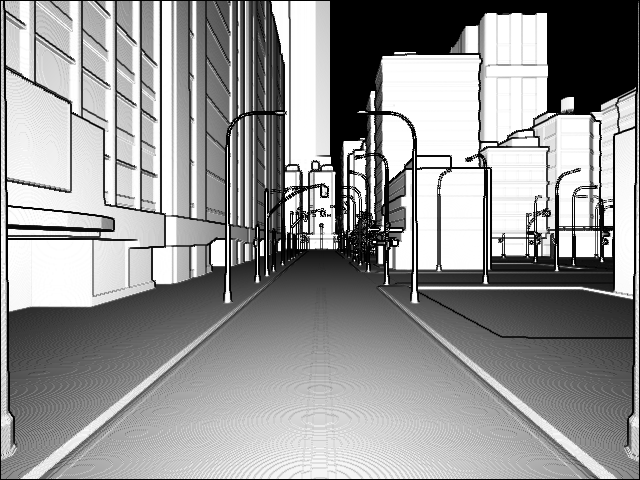
\includegraphics[width=0.24\linewidth]{chapterB/odometry/flexion_0200.png}%
    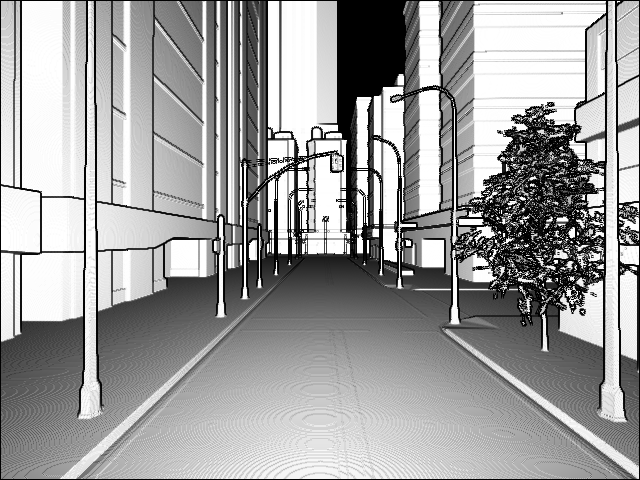
\includegraphics[width=0.24\linewidth]{chapterB/odometry/flexion_0350.png}%
    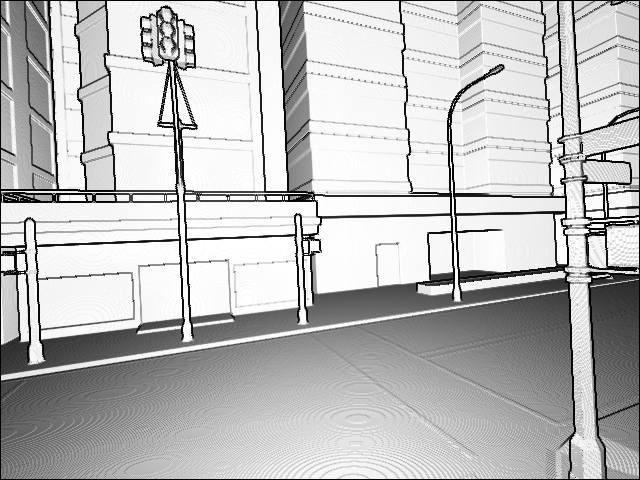
\includegraphics[width=0.24\linewidth]{chapterB/odometry/flexion_1290.png}%
    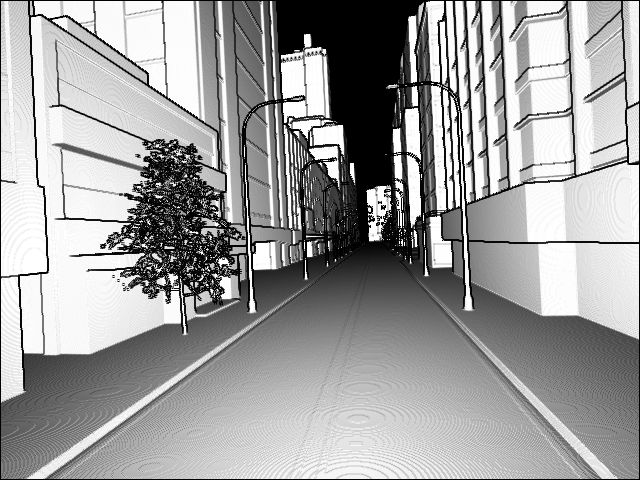
\includegraphics[width=0.24\linewidth]{chapterB/odometry/flexion_2100.png}\\
    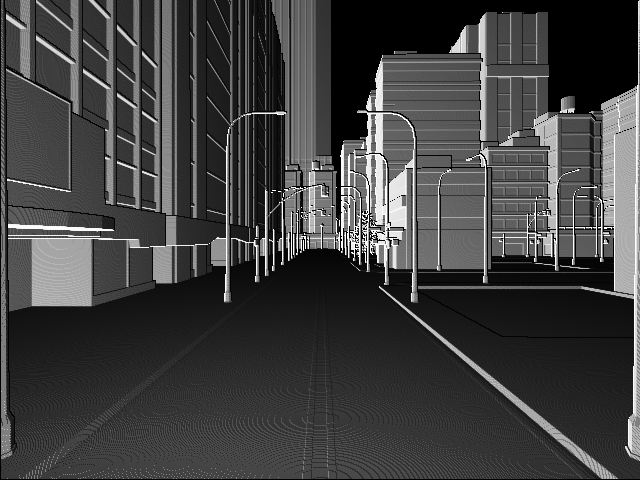
\includegraphics[width=0.24\linewidth]{chapterB/odometry/bearing_0200.png}%
    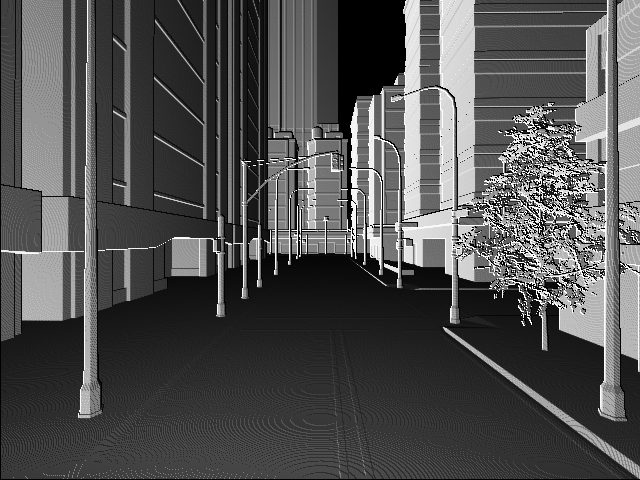
\includegraphics[width=0.24\linewidth]{chapterB/odometry/bearing_0350.png}%
    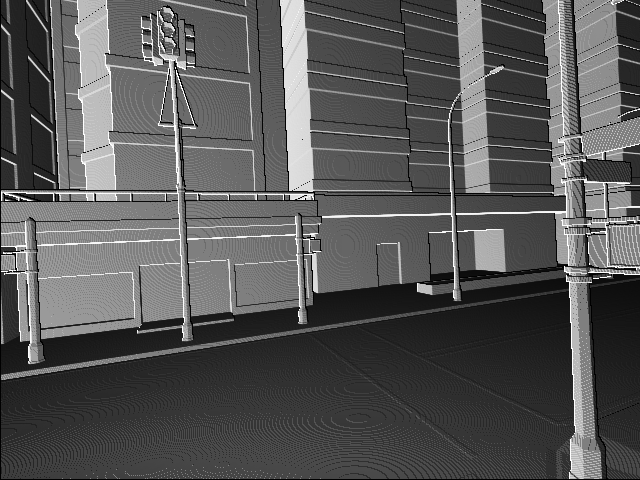
\includegraphics[width=0.24\linewidth]{chapterB/odometry/bearing_1290.png}%
    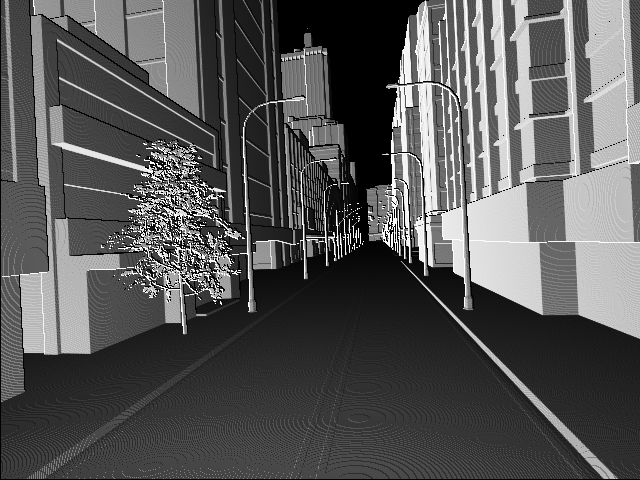
\includegraphics[width=0.24\linewidth]{chapterB/odometry/bearing_2100.png}\\
    \caption{\glspl{flexion-image} and \glspl{bearing-angle-image} for the \emph{Odometry} dataset.}
\end{figure}
